\documentclass[tikz,convert={outfile=images/monoid-in-moncat-unitality.png,density=1000}]{standalone}
\usepackage[build={latexoptions={-output-directory=latex/png}}]{standalone}
\tikzset{
  ->/.style={draw=white!50!black,-stealth}
}
\tikzstyle{every node}=[color=white!50!black,font=\footnotesize]
\begin{document}
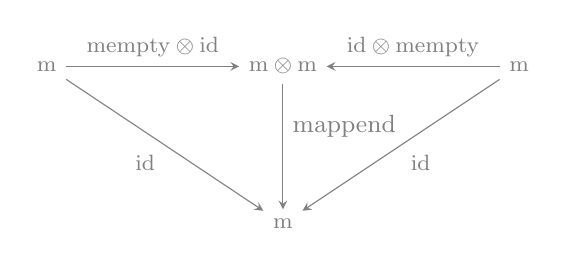
\begin{tikzpicture}
    \node (A) at (0,2) {\(\mathrm{m}\)};
    \node (B) at (3,2) {\(\mathrm{m\otimes m}\)};
    \node (C) at (6,2) {\(\mathrm{m}\)};
    \node (D) at (3,0) {\(\mathrm{m}\)};
    \draw [->] (A) -- node[above] {\(\mathrm{mempty\otimes id}\)} (B); 
    \draw [->] (C) -- node[above] {\(\mathrm{id\otimes mempty}\)} (B);
    \draw [->] (B) -- node[above right] {\small\(\mathrm{mappend}\)}  (D);
    \draw [->] (A) -- node[below left]  {\(\mathrm{id}\)} (D);
    \draw [->] (C) -- node[below right] {\(\mathrm{id}\)} (D);
\end{tikzpicture}
\end{document}
